\chapter{Gennemgang af kode}
\section{Frontend}
\subsection{Pakke visning}

\begin{figure}[h]
    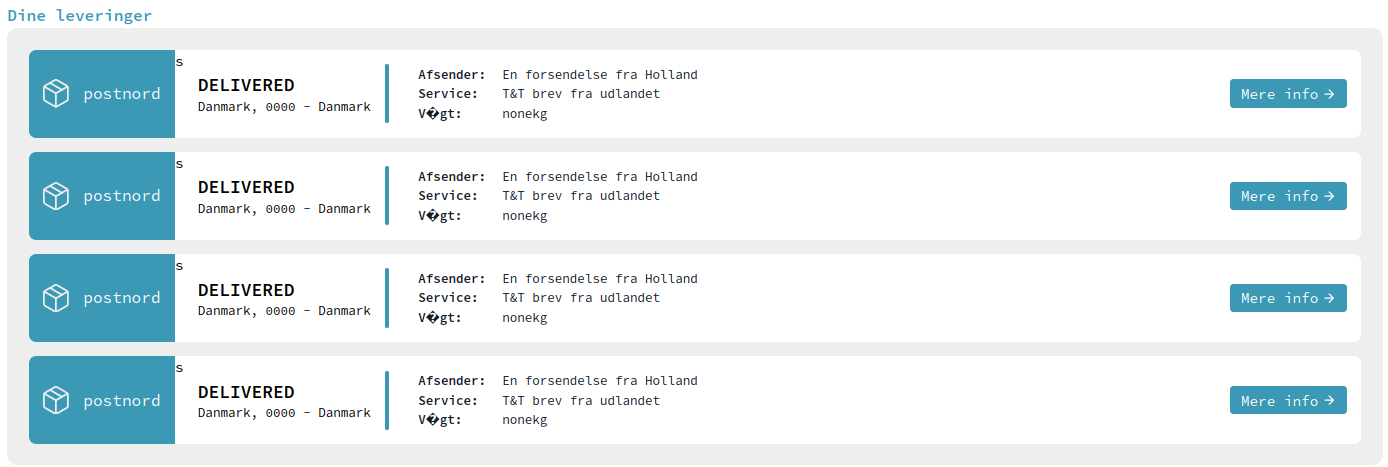
\includegraphics[scale=0.35]{./Pictures/PakkeView.png}
    \centering
    \caption{Pakke visning.}
     \label{fig:PakkeView}
  \end{figure}

\begin{figure}[!h]
    \begin{minted}[frame=lines,framesep=2mm,baselinestretch=1.2,linenos]{cs}
        @model PackageTrackingApp.Viewmodels.MyPageVM;
        @{
            int iteration = 0;

            foreach(var package in Model.shipments) {

                iteration++;

                string boksId = $"box{iteration}";
             
            // Her ligger alt koden til at fremstille Pakke visning
                
            }
        }
    \end{minted}
\caption{Shipments.cshtml}

\label{code:Shipments.cs}
\end{figure}

Dette er koden der genere hver boks som viser hvilke pakker man har i ens email se figur 5.1. Vi starter med at 
definere modellen MyPageVM som indeholder data om ens pakker, som bliver generet i HomeControlleren.
Herefter laver vi en variabel der indeholder tal som skal indexe hvilke pakke den er nået til. Der er så 
et foreach løkke som for hvert element i Modellen shipments er en variabel "package" som indeholder information
om pakken. Så bliver iteration plusset en til. der bliver så deklareret "boksId" streng som er ligmed en streng interpolation
hvor "box" sættes sammen med "iteration" nummeret. under dette ligger der så en masse kode der ikke var plads til i opgaven.
\newpage
\begin{figure}[!h]
    \begin{minted}[frame=lines,framesep=1.8mm,baselinestretch=1,linenos]{cs}
<div class="bg-white rounded-lg flex flex-row" style="visibility: flex;" id="@boksId">
<div class="bg-primaryBlue rounded-l-lg h-auto p-4 flex flex-col md:flex-row items-center mx-auto">
    <h1 class="text-sm md:text-lg text-white">@package.info.courrier</h1>
</div>
<div class="w-full p-4 rounded-r-lg flex flex-row space-x-4">
    <div class="flex flex-col my-auto">
        <h1 class="text-xl font-semibold">@package.currentStatus</h1>
                @{
                    string currntEventLocationtxt = package.events.Last().location.city + ", " 
                    + @package.events.Last().location.zipCode + " - " 
                    + @package.events.Last().location.country;
                }
                <h1 class="text-sm">@currntEventLocationtxt</h1>
    </div>
    <div class="h-full bg-none md:bg-primaryBlue rounded-full w-1 flex-grow md:flex-initial"></div>
    <div class="flex-grow hidden md:block">
        <table class="table-auto border-separate border-spacing-x-4 text-sm text-gray-900">
            <tr class="mx-4">
                <td class="font-semibold">Afsender:</td>
                <td>@package.info.consignor.name</td>
            </tr>
            <tr>
                <td class="font-semibold">Service:</td>
                <td>@package.info.service</td>
            </tr>
            <tr class="">
                <td class="font-semibold">Vægt:</td>
                        @{string weight = package.info.weight + "kg";}
                <td>@weight</td>
            </tr>
        </table>
    </div>
    <div class="my-auto items-center float-right" >
                <a class="btn-primary" onclick="moreInfo(@iteration)">
            <p>Mere info</p>
        </a>
    </div></div></div>
\end{minted}
\caption{Shipments.cshtml}
\label{code:Shipments.cs}
\end{figure}

Dette kode er inde i foreach løkken. på linje 2 har vi et div html tag som definere en division af koden.
Som indpakker h1 tagget på linje 3 hvor teksten er sat til at være variabellen "package.info.courrier" som er 
inde i h1 tagget. div'en rundt om bruger klasserne "bg-primaryBlue", "rounded-l-lg", og "h-auto" Dette gør at baggrundsfarven er blå
og har afrundet hjørner til venstre. 

på linje 5-6 er der to nye div html tags. det her er den hvide del af hver pakke kasse. Klassen "w-full"
gør at boksen fylder 100\% af kontaineren. klasserne "flex" og "flex-row" laver elementet til en fleksibel kontaineren. klasserne "p-4" og "space-x-4"
først giver vi elementet en padding på 4. Derefter tilføjes der en margen på 4 mellem elementerne som er mellemrummet mellem elementerne. klassen "rounded-r-lg" gør
at elementet har afrundet med en stor radius. det andet div element på linje 6 bruger klasserne "flex flex-col my-auto".
Dette gør Ddette element til en fleksibel container med en enkelt kolonne, der justeres centralt i en vandret linje af det primære element.
"my-auto" klassen justere elementerne vertikalt så det er i midten af det primære element på linje 5. inde i det sekundære div-element bruges h1 tag 
til at lave en tekst med pakkes status her bruges klasserne "text-xl font-semibold" som gør at teksten er stor og fremhævet. under dette bruges 
der razor-syntaks til at lave en teskt. der bliver lavet en streng hvor flere varialer bliver plusset sammen til en streng.
Herefter bliver denne her variabel brugt i et h1 tag med klassen "text-sm" som gør teksten lille. 

På linje 15 laves et div-element som laver en blå vandret streg med runde hjørner som deler information delene i to.
Derefter er der et div-element med klasserne "flex-grow hidden md:block" hidden gør at dette element er skjult men kun på små skærme
ved brug af klassen "md:block". Derefter laves et table element  med klasserne "table-auto border-separate border-spacing-x-4 text-sm text-gray-900"
som gør at tablen selv justere sig til dens indhold. "border-separate" og "border-spacing-x-4" gør at der er en synlig grænse mellem hver celle hvor der er
en afstand på 4 pixels mellem grænserne. "text-sm" gør at teksten i felterne er i en mindre skriftstørrelse, , og "text-gray-900" 
klassen angiver, at teksten skal være mørkegrå. Herefter angives der en tabelrække med "tr" elementet som bruger klassen "mx-4" som laver en vandret margen.
inde i dette element er der så to celler defineret med elementet "td". på linje 19 laves en celle hvor der står "Afsender" med en halv fed skrifttype.
Der er så et celle mere hvor der indsættes en navn på afsenderen ved hjælp af objektet "package.info.consignor.name". der bliver så lavet to rækker mere med
andre informationer.

på linje 33 er der et div element med klasserne "my-auto items-center float-right" dette gør at elementet bliver centreret i kontaineren og både horisonalt og vertikalt.
"float-right" placerer element i højre side af kontaineren. inden i dette element er der et a link element med klassen "btn-primary" som gør at elementet 
har stilet som en knap. dette element bruger så "onclick="moreInfo(@iteration)" hvor angiver en JavaScript-funktion, der køres, når knappen klikkes på. I dette tilfælde vil funktionen "moreInfo" 
køres, og @iteration vil blive sendt som et argument til funktionen. Denne funktion vil folde boksen ud med mere information om pakke leveringen. inde i a elementet 
er der så et p element hvor der står "Mere info". Dette er vist som synlig tekst på knappen.





\section{Backend}
\subsection{Oprettelse af Konto}
\newpage
\begin{figure}[!ht]
    \begin{minted}[frame=lines,framesep=2mm,baselinestretch=1.2,linenos]{cs}
        // denne funktion sender en Email med sendgrid ved at bruge sendgrids smtp server.
        public async Task SendEmailAsync(string toEmail, string subject, string message)
        {
            var apiKey = "----------------------------------"; // sendgrid api key
            await Execute(apiKey, subject, message, toEmail);
        }
    
        public async Task Execute(string apiKey, string subject, string message, string toEmail)
        {
            _logger.LogInformation(apiKey);
            var client = new SendGridClient(apiKey);
            var msg = new SendGridMessage()
            {
                From = new EmailAddress("mads.gjellerod@gmail.com", "Password Recovery"),
                Subject = subject,
                PlainTextContent = message,
                HtmlContent = message
            };
            msg.AddTo(new EmailAddress(toEmail));
            // fjerner klik tracking fra koden 
            msg.SetClickTracking(false, false);
            var response = await client.SendEmailAsync(msg);
            // sennder en besked til konsollen til at debug evtuelle fejl
            _logger.LogInformation(response.IsSuccessStatusCode
                                   ? $"Email to {toEmail} queued successfully!"
                                   : $"Failure Email to {toEmail}");
        }
    \end{minted}
\caption{EmailSender.cs}\label{code:EmailSender.cs}
\end{figure}

Dette er koden der sender en email når man eksempelvis registere sig på siden og skal 
konfirmitere ens email. når man vil sende en email i programmet kalder man metoden SendEmailAsync.
Denne metode har signature af at være public hvilket betyder at andre metoder kan kalde den. Så har
den også signaturene "async Task" som gør at metoden gøre parrelet med andre opgaver så når man venter på
en Api response så stopper programmet ikke. Denne metode tager tre paramatere som er strege af tekst.
Det første der sker i metoden er at vi laver en variabel der indeholder vores "Sendgrid" api key.
herefter laves der et kaldt til metoden Execute som bliver kaldt asynkront ved hjælp af "await" operatøren.

I Execute metoden bliver der først oprettet et instans af SendGridClient som indeholder api nøglen.
Derefter bliver der lavet et instans af Klassen SendGridMessage som kaldes msg som bruges til at opbygge. 
Beskenden som skal sendes. Her bliver der sat nogle variabler som hvem den er fra og beskendens indhold. 
den næste er at metoden AddTo bliver brugt til at sætte emailen som beskenden skal sendes til. Herefter bruges metoden 
SetClickTracking som der gives to false værdier til at deaktivere Click tracking. først defineres der en implicit variabel 
som kaldes "response" som vil være den type som der returneres fra SendEmailAsync metoden. Der bruges "await" operatøren som venter
på at metoden fuldfører udførelsen, før koden fortsætter med at køre. client er et objekt af typen SendGridClient som har metoden
SendEmailAsync som er en asynkron metode.
\bigbreak
\noindent
Dette er metoden der bruges når der skal laves en ny bruger. Denne funktion bliver kaldt når brugeren har trykker registere på hjemmesiden eller
når brugeren logge ind med en ny Google konto. når denne metode bliver kaldt kører metoden asynkront i baggrunden.

\begin{figure}[!h]
    \begin{minted}[frame=lines,framesep=1.8mm,baselinestretch=1,linenos]{cs}
public async Task<IActionResult> OnPostAsync(string returnUrl = null)
{
    // her sættes hvilke url der skal bruges når registeringen er færdig
    returnUrl ??= Url.Content("~/");
    // her henter den en liste af andre logins
    ExternalLogins = (await _signInManager.GetExternalAuthenticationSchemesAsync()).ToList();
    // hvis dette er okay går den videre
    if (ModelState.IsValid)
    {
        // bruger metoden RegisterModel.CreateUser til at lave en model for registeringen
        var user = CreateUser();
        // her gemmer vi data brugeren har sat i felterne i databasen
        await _userStore.SetUserNameAsync(user, Input.Email, CancellationToken.None);
        await _emailStore.SetEmailAsync(user, Input.Email, CancellationToken.None);
        
        var result = await _userManager.CreateAsync(user, Input.Password);
\end{minted}
\caption{Register.cshtml.cs}\label{code:Register.cshtml.cs}
\end{figure}
Dette første vi gør i metoden. er at sætte variablen returnUrl hvis den er null dette gøres ved at bruges "??=" som er 
en sammensat operatør som kun tildeller en værdi hvis værdien af variablen er null. Herefter på linje 6 bliver der initialiseret en liste
af eksterne login metoder der er tilgængelige for brugerne. Til dette bruges "\_signInManager" som er en feltvariabel af typen "SignInManager<IdentityUser>"
som er en klasse i Identity framework. Metoden "GetExternalAuthenticationSchemesAsync" bliver så brugt til at returnere alle tilgængelige eksterne login metode. 
Dette bliver så lavet til en liste ved at bruge metoden "ToList". 

Det der så sker er at vi tjekke om "ModelState" er gyldig dette er den ved at der ikke er sket nogle fejl
i programmet. Den her "ModelState" er en egenskab i ASP.NET Core som indeholder en samling af fejl som 
kunne være under sket under at data er blevet konveteret til modeller. Hvis så "ModelState" er gyldig bliver der
først lavet en variabel "user" hvor metoden "CreateUser" som laver en ny bruger model. 

Herefter gemmes bruges navn og email. Ved at bruge "\_userStore" og "\_emailStore" bliver instansiliseret længere oppe i koden det her instans af "IUserStore" og "IUserEmailStore".
Her bruges metoderne "SetUserNameAsync" og "SendEmailAsync" som gemmer dette i databasen. disse metoder tager tre paramatere ind. først tager
den en model for registering af bruger som var den variabel vi kaldte "user". I anden paramatere tager metoden "SetUserNameAsync" et navn som input.
Hvor "SetEmailAsync" tager en email begge paramatere her er sat til variablen "Input.Email" da ens navn som bruger er ens email den "Input" klasse indeholder data fra formdata fra registering siden. Den sidste paramatere som metoderne 
tager ind er "CancellationToken" den er sat til none da webapplicationen ikke gøre brug af det, men denne token kan bruges til at afbryde registering hvis der sker en fejl
eller at forbindelsen til databasen forsvinder. Herefter bruges et instans af klassen "UserManager" hvor metoden "CreateAsync" bliver
brugt til at lave en ny bruger i databasen. den tager "user" variablen og et kodeord som paramatere. 
\newpage

\begin{figure}[!h]
    \begin{minted}[frame=lines,framesep=1.8mm,baselinestretch=1,linenos]{cs}
        // hvis bruger kunne laves kører koden videre 
        if (result.Succeeded)
        {
            // dette er til at debug problemer i koden
            _logger.LogInformation("User created a new account with password.");
            // her laver vi en variabel med bruges id som vi lavet før.
            var userId = await _userManager.GetUserIdAsync(user);
            // her generere vi en token som bruges når brugeren skal konfimere sin email
            var code = await _userManager.GenerateEmailConfirmationTokenAsync(user);
            // vi kryptere så denne token med Base64 encoding.
            code = WebEncoders.Base64UrlEncode(Encoding.UTF8.GetBytes(code));
            // her efter laves en ny midlertidig side hvor konfimationen af emailen ventes på
            var callbackUrl = Url.Page(
                "/Account/ConfirmEmail",
                pageHandler: null,
                values: new { area = "Identity", userId = userId, code = code, returnUrl = returnUrl },
                protocol: Request.Scheme);
            // her bliver emailen sendt med linkent til den nye midlertidig side.
            await _emailSender.SendEmailAsync(Input.Email, "Confirm your email",
                $"Please confirm your account by <a href='{HtmlEncoder.Default.Encode(callbackUrl)}'>clicking here</a>.");
            // her tjekkes om brugeren har accepteret sin email.
            if (_userManager.Options.SignIn.RequireConfirmedAccount)
            {
                // her bliver brugeren diageret til forsiden
                return RedirectToPage("RegisterConfirmation", new { email = Input.Email, returnUrl = returnUrl });
            }
            else
            {
                // hvis ikke emailen bliver konfirmation vil den ikke virke
                await _signInManager.SignInAsync(user, isPersistent: false);
                // her bliver brugeren diageret til forsiden
                return LocalRedirect(returnUrl);
            }

        }
        // Hvis koden når her til er noget fejlet under registering af bruger.
        return Page();
\end{minted}
\caption{Register.cshtml.cs}\label{code:Register.cshtml.cs}
\end{figure}

Hvis så resultatet af "\_userManager.CreateAsync" er "Succeeded" vil koden kører videre. Det første
der sker er at der bliver sendt en besked til consolen til at debug applicationen. Derefter laves der 
en variabel "userId" som henter et user id fra objektet "user" ved hjælp af metoden "GetUserIdAsync" som er en metode der kører asynkront.
her generere vi en token som bruges når brugeren skal konfimere sin email ved hjælp af metoden "GenerateEmailConfirmationTokenAsync".
derefter bliver token kryptere med base64 encoding. På linje 13 bliver der så lavet en ny side der bruger stien "Account/ConfirmEmail".
Derefter bliver emailen sendt ved hjælp af EmailSender.cs på figur 5.4 ved hjælp af metoden "SendEmailAsync" som kører asynkront. Denne metode 
tager tre parameter ind først er det hvilken email beskeden skal sendes til. Herefter Emnet og til sidst selve beskeden som i dette tilfælde
er linket til at acceptere sin mail. på linje 22 tjekkes der så om mailen er blevet accepteret ved at kalde metoden "RequireConfirmedAccount" som
returnere en boolean. hvis det så er sandt vil metoden returnere en  "RedirectToPage" til "RegisterConfirmation". Ellers bliver brugers konto slettet og
brugeren bliver sendt til forsiden. 